% Drawing 148/02-4 -- folder 148, batch 02, archive page 22 (PDF page 23).
% Transcription: en bas à droite, au-dessus du cadre, un quadrillage carré avec des diagonales ; un point central marqué, d'où partent un trait horizontal et un trait vertical repassés en gras.
% Kind: square grid with diagonals and a marked central point. Method 2 (redrawn stroke by stroke from the facsimile). Status: ok.
% Notes: Ink, overdrawn, on the ruled paper above the frame of the diagram below. Redrawn stroke by stroke on 2026-11-14 (issue 147, second pass, Claude Opus 5.5) from the 400 dpi scan, every stroke through points read on a crop gridded every two units; the bbox is lowered to 0.765 so that the lower ends of the verticals and the two short strokes at the foot are whole. Drawn as on the page: the left vertical of the upper part and, a little to its left, the long left vertical of the lower part; the long vertical through the middle left, with the short foot stroke across its lower end; the heavy centre vertical from the top down through the heavy point and on, thinner, to its hooked lower end, with the second faint stroke beside its upper part; the vertical from the top of the right N down to its arrow-like end, with the short barb; the right side of the upper rectangle and the doubled right vertical of the lower part; the top side from the blot at the top of the centre vertical, the short hooked stroke and the curved stroke at the top left; four horizontals at their own heights, the second heavy from about the middle left vertical to near the right side; the diagonals as they run on the page: from the top left corner to the centre, the long one from the left below the heavy horizontal to the lower middle, the short one under it, the two of the upper middle cells, the N at the upper right with the hook and the diagonal in the cell under it, the heavy stroke from the top right of the centre down to the heavy horizontal and the thin one beside it, the thin cross in the cell left of the centre, the cross below the centre (one stroke heavy and short), the stroke to the lower right corner, the turned corner at the right end of the heavy horizontal; the two small ticks and the blot in the cells. Overlay: rasterised by the local TikZ interpreter (not compiled: no TeX in the session) and laid over the 400 dpi colour scan; every stroke lies on its ink to within about one unit. Earlier redraws (2026-11-12, 2026-11-13) drew a regular four-by-four grid that was up to three units off the page and had diagonals the page does not have; that is gone.
% Coordinates: 1 unit = 1 mm = 1/100 of the crop width, y downwards as on the crop (bbox in page fractions: [0.63, 0.64, 0.83, 0.765]).
% Redrawn by Claude (claude-fable-5-2), issue #128, 2026-11-12; not checked by a human; not compiled (no TeX in the session); overlay-checked on the scan by Claude Opus 5.5, issue #147, 2026-11-13, not compiled (no TeX in the session).
% Rights: reproduces part of the work -- behind RENDER_TRANSCRIPTS, never published by itself.
\documentclass[tikz,border=3pt]{standalone}
\usepackage{amsmath,amssymb}
\usetikzlibrary{patterns,arrows.meta}
\tikzset{pencil/.style={black!45}, struck/.style={black!35}, mpt/.style={circle,draw,inner sep=1.3pt}, pt/.style={circle,fill,inner sep=0.9pt}, opt/.style={circle,draw,fill=white,inner sep=1.1pt}, Rd/.style={red!75!black}, Gn/.style={green!45!black}, Br/.style={brown!70!black}}
\begin{document}
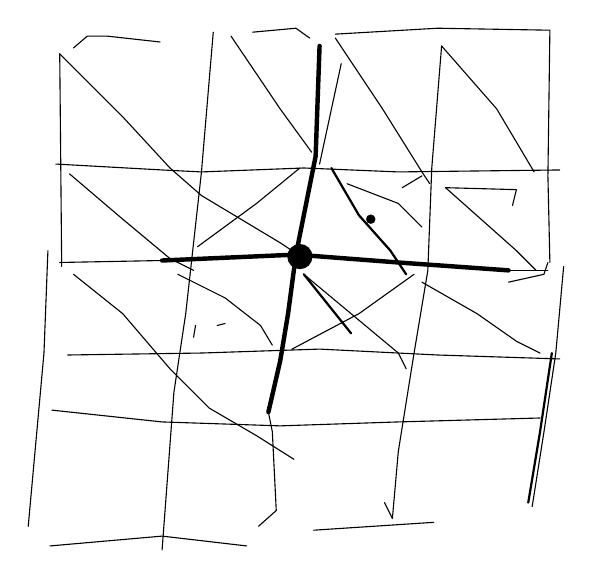
\begin{tikzpicture}[x=1mm,y=-1mm,line cap=round,line join=round,font=\small]
\draw (27,22) -- (27.25,49);
\draw (28.75,21.25) -- (30.5,19.75) -- (33,19.75) -- (39.75,20.5);
\draw (27,22) -- (35,30) -- (41,36.5) -- (45,40) -- (50,43) -- (55,46) -- (56.5,47);
\draw (26.5,36) -- (40,36.75) -- (45,37) -- (58,36.5) -- (70,37) -- (90.5,36.75);
\draw (46.5,19.25) -- (45,37) -- (44,46) -- (43,55) -- (41.5,65) -- (40,85);
\draw (25.75,84.5) -- (40,83.25) -- (50.75,84.5);
\draw (25.5,47) -- (25,60) -- (23,82);
\draw (28.25,37.25) -- (35,43) -- (41,48) -- (44,49.5);
\draw (27,48.5) -- (40,48.25);
\draw[line width=1.6pt] (40,48.25) -- (57,47.5) -- (70,48.5) -- (84,49.5);
\draw (84,49.5) -- (89,49.5);
\draw[line width=1.6pt] (60,21) -- (59.5,35) -- (58,42.5) -- (57,47.5) -- (56,55) -- (55,61) -- (53.5,67.5);
\draw (53.5,67.5) -- (54,70) -- (54.5,80) -- (52.25,82);
\draw (48.75,19.75) -- (55,29) -- (59,34.5);
\draw (51.5,19.25) -- (57,18.75) -- (58.75,20);
\draw (62,19.5) -- (75,18.75) -- (89.25,19) -- (89,37.5) -- (89.25,48.5);
\draw (62,20) -- (68,29) -- (73,37) -- (74,38.5);
\draw (62.75,23.25) -- (60,36);
\draw (75.5,21) -- (74.25,36.5) -- (73.75,49.5) -- (72,60) -- (70,72.5) -- (69.25,81);
\draw (68.25,79) -- (69.25,81);
\draw (75.5,21) -- (82.5,29) -- (87.25,37);
\draw (70.5,39) -- (73,37.5);
\draw (76,39) -- (85,39.25) -- (84.5,41.25);
\draw (76,39) -- (85,47) -- (87.5,49.5);
\draw (89,48.5) -- (88.5,50) -- (84,51);
\draw[thick] (61.5,36.5) -- (65,42.5) -- (69,47) -- (71,50);
\draw (63.5,38.5) -- (70,41) -- (73,44);
\draw (44.5,46.5) -- (52,41) -- (57.5,36.5);
\draw[thick] (58,50) -- (64,57.5);
\draw (58,50) -- (70,60) -- (71,62);
\draw (72,50) -- (65,55) -- (56.5,59.5);
\draw (73,51) -- (80,55) -- (85,58.5) -- (88,60);
\draw (28.75,50) -- (35,55) -- (41,62) -- (46,67) -- (52,70.5) -- (56.75,73.5);
\draw (42,50) -- (48,53) -- (52.5,56.5) -- (54,59);
\draw (28,60.25) -- (45,60) -- (60,59.5) -- (75,60.25) -- (90.5,60.75);
\draw (26,67.25) -- (40,68.75) -- (55,69.25) -- (70,68.75) -- (88,68.25);
\draw (91,49) -- (90,60) -- (88.5,70) -- (87,79.5);
\draw[thick] (89.5,60) -- (88,70) -- (86.5,79);
\draw (59.25,82.5) -- (74.5,81.5);
\draw (44,58) -- (44.25,56.5);
\draw (47,56.5) -- (48,56.25);
\fill (66.5,43) circle [radius=0.6];
\fill (57.5,47.75) circle [radius=1.6];
\end{tikzpicture}
\end{document}
